\section{Memento-Muster}

\subsection{Problemstellung}
Sie entwickeln ein Computerspiel und sollen eine Speichern-Funktionalit"at hinzuf"ugen, die die Spielfigur zu einem sp"ateren Zeitpunkt an den gespeicherten Platz zur"uck bef"ordert falls dieser im sp"ateren Spielverlauf etwas zusto"sen sollte.

\subsection{Erkl"arung des Musters}
\textbf{Definition:} Verwenden Sie das Memento-Muster, wenn es erforderlich ist, dass Sie ein Objekt in einen seiner fr"uheren Zust"ande zur"ucksetzen k"onnen, z.B. wenn Ihr Benutzer die Anweisung \emph{r"uckg"angig} eingibt.

\textbf{Ziele des Musters:} Das Memento/Muster hat zwei Ziele
\begin{itemize}
	\item Den wichtigen Zustand des Schl"ussel-Objekts von einem System speichern.
	\item Die Kapselung des Schl"ussel-Objekts bewharen.
\end{itemize}

Vor dem Hintergrund des Prinzips \emph{nur eine Zust"andigkeit pro Klasse} ist es auch eine gute Idee, den zu speichernden Zustand von dem Schl"ussel-Objekt zu trennen. Dieses separate Objekt, das den Zustand h"alt, wird Memento-Objekt genannt. 

\subsection{Vor/Nachteile}

\textbf{Vorteile des Memento-Musters:}
\begin{itemize}
	\item Wenn der gespeicherte Zustand au"serhalb des Schl"usselobjekts gehalten wird, bleibt die Koh"asion \emph{(innerer Zusammenhalt)} erhalten.
	\item Bewahrt die Kapselung der Daten des Schl"ussel-Objekts.
	\item Bietet eine leicht zu implementierende Wiederherstellungsm"oglichkeit. 
\end{itemize}


\textbf{Verwendung und Nachteile:}
\begin{itemize}
	\item Das Memento-Muster wird zur Speicherung eines Zustands verwendet.
	\item Speicherung und Wiederherstellung k"onnen zeitaufwendig sein.
	\item In Java-Szstemen sollten Sie in betracht ziehen, Systemzust"ande stattdessen "uber Serialisierung zu speichern. 
\end{itemize}

\begin{figure}
	\centering
	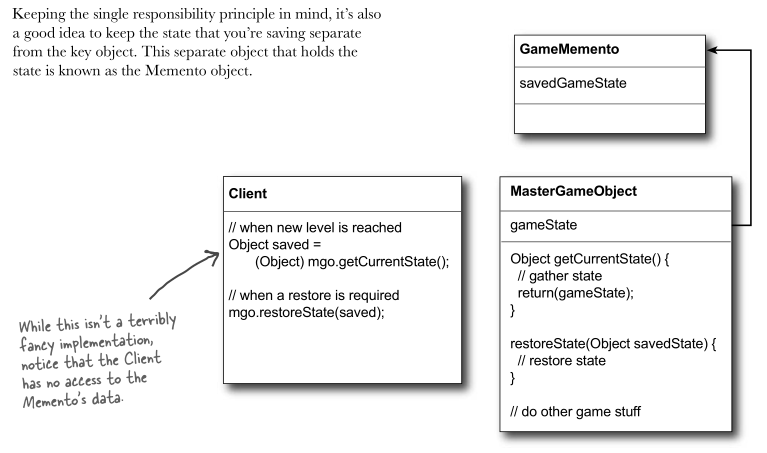
\includegraphics[width=.9\linewidth]{memento/img/mementoUML}
	\caption{UML-Darstellung des Memento-Musters}
	\label{fig:mementoUML}
\end{figure}
